\documentclass[a4paper,12pt]{article}
\usepackage[utf8]{inputenc}
\usepackage{graphicx}
\usepackage{caption}
\usepackage{booktabs}
\usepackage{array}
\usepackage{amsmath}
\usepackage{amsfonts}
\usepackage{hyperref}
\usepackage{xcolor}
\usepackage{float}
\usepackage{booktabs}   % For professional-looking tables
\usepackage{multirow}   % For merged rows
\usepackage{float}      % For precise table positioning with [H]
\usepackage[a4paper, margin=1in]{geometry}

\title{Part 1 :Digit Classification on Reduced MNIST Dataset Using MLP and CNN}

\begin{document}

\maketitle

\section{Introduction}
The reduced MNIST dataset, a subset of the MNIST dataset, consists of 1000 training examples and 200 testing examples per digit (0-9), with images of size 28 x 28 pixels in grayscale. This assignment is divided into two parts:

\begin{itemize}
    \item \textbf{Part 1 (MLP with Feature Extraction):} Implement an MLP with 1, 3, or 5 hidden layers, using features extracted by Principal Component Analysis (PCA), Discrete Cosine Transform (DCT), and Autoencoders (AE).
    \item \textbf{Part 2 (CNN with LeNet-5 variants):} Train a CNN based on the LeNet-5 architecture, adjust the structure to fit 28x28 images, and explore at least two variations in hyperparameters.
\end{itemize}

The objective is to compare the performance of these models in terms of accuracy, training time, and testing time, and to provide information on the impact of architectural choices.

\section{Methodology}

\subsection{Dataset}
The reduced MNIST dataset contains:
\begin{itemize}
    \item \textbf{Training Set:} 1000 examples per digit (10,000 total).
    \item \textbf{Testing Set:} 200 examples per digit (2,000 total).
\end{itemize}
The images are 28x28 pixels in grayscale and the labels correspond to digits 0-9.

\subsection{Part 1: Multi-Layer Perceptron (MLP) with Feature Extraction}
In this part, we implemented an MLP with 1, 2, and 3 hidden layers, using features extracted from the images via three methods:
\begin{itemize}
    \item \textbf{PCA:} Reduced dimensionality while retaining 95\% variance.
    \item \textbf{DCT:} Extracted frequency-based features (225 components).
    \item \textbf{Autoencoder (AE):} Learned a compressed representation (225 components) using an encoder-decoder network.
\end{itemize}
The MLP architectures were trained for 40 epochs with a batch size of 64, using the Adam optimizer.

\subsection{Part 2: Convolutional Neural Network (CNN) with LeNet-5 variants}
We implemented a CNN based on the LeNet-5 architecture, adjusted for 28x28 images. The base model consists of the following.
\begin{itemize}
    \item Two convolutional layers (6 and 16 filters, 5x5 kernels, ReLU activation).
    \item Average pooling layers (2x2, stride 2).
    \item Three fully connected layers (120, 84, and 10 units, with ReLU for hidden layers and softmax for output).
\end{itemize}
The model was trained for 40 epochs with a batch size of 64, using the Adam optimizer (except where specified). We explored the following variations:
\begin{itemize}
    \item \textbf{Variation 1 (Increased Filters):} Increased the number of filters to 18 and 24 in the convolutional layers.
    \item \textbf{Variation 2 (Tanh Activation):} Used tanh activation instead of ReLU.
    \item \textbf{Variation 3 (ELU Activation):} Used ELU activation instead of ReLU.
    \item \textbf{Variation 4 (Fewer Layers):} Removed one dense layer (120 units).
    \item \textbf{Variation 5 (Additional Layer):} Added a dense layer (42 units).
    \item \textbf{Variation 6 (MaxPooling):} Replaced AveragePooling with MaxPooling.
    \item \textbf{Variation 7 (Dropout):} Added dropout layers for regularization (0.25 after convolutional layers, 0.5 after the first dense layer).
    \item \textbf{Variation 8 (Batch Normalization):} Added batch normalization after convolutional and dense layers.
    \item \textbf{Variation 9 (SGD Optimizer):} Used SGD with momentum (learning rate 0.01, momentum 0.9) instead of Adam.
    \item \textbf{Variation 10 (Smaller Kernel):} Used 3 x 3 kernels instead of 5 x 5.
\end{itemize}

\section{Results}

\subsection{Part 1: MLP with Feature Extraction}
The MLP models were trained with 1, 2, and 3 hidden layers, using features extracted via PCA, DCT, and Autoencoder. The results for each configuration are presented below, along with specific observations and comments.

\begin{figure}[H]
    \centering
    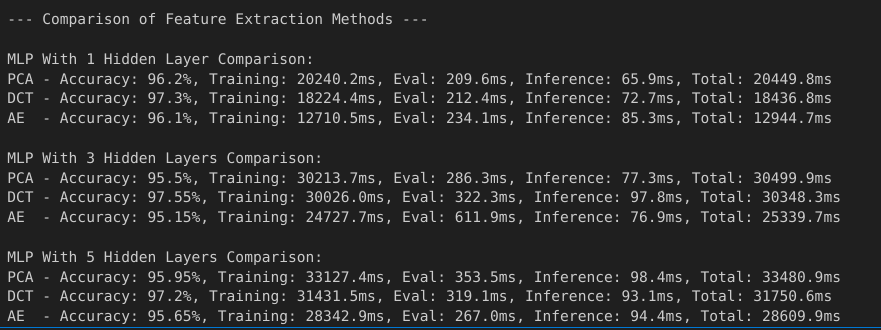
\includegraphics[width=0.8\textwidth]{MLPlayers.png}
    \caption{MLP with 1,3,5 Hidden Layer: Comparison of PCA, DCT, and Autoencoder.}
    \label{fig:mlp_1_hidden}
\end{figure}

\textbf{Observations and Comments for MLP with 1 Hidden Layer:}
\begin{itemize}
    \item \textbf{Accuracy:} DCT achieved the highest accuracy at 97.2\%, followed by PCA at 95.6\%, and Autoencoder at 93.55\%. This suggests that DCT features are particularly effective for simpler MLP architectures, likely due to their ability to capture frequency-based patterns in the data.
    \item \textbf{Training Time:} DCT was the fastest to train (14.8s), compared to PCA (20.3s) and Autoencoder (16.1s). The shorter training time for DCT may be attributed to its efficient feature representation, which reduces the computational burden on the MLP.
    \item \textbf{Inference Time:} Inference times were similar across all methods, with PCA at 65.9ms, Autoencoder at 66.7ms, and DCT at 69.8ms. This indicates that the choice of feature extraction method has a minimal impact on inference speed for a single hidden layer.
    \item \textbf{Comment:} The superior performance of DCT in both accuracy and training time makes it the preferred feature extraction method for a 1-hidden-layer MLP. Autoencoder's lower accuracy suggests that the learned features may not be as discriminative for this task.
\end{itemize}

\textbf{Observations and Comments for MLP with 2 Hidden Layers:}
\begin{itemize}
    \item \textbf{Accuracy:} DCT again outperformed the others with an accuracy of 97.35\%, slightly better than its 1-hidden-layer performance. PCA achieved 95.55\%, nearly identical to its 1-hidden-layer result, while Autoencoder improved slightly to 93.8\%. The marginal improvement in DCT's accuracy suggests that adding a second hidden layer enhances its ability to model complex patterns in the frequency domain.
    \item \textbf{Training Time:} Training times increased for all methods due to the additional layer: DCT took 22.4s, PCA 28.0s, and Autoencoder 24.4s. PCA's training time increased the most, indicating that its features may require more computation to process through deeper networks.
    \item \textbf{Inference Time:} Inference times also increased slightly, with DCT at 71.8ms, PCA at 68.0ms, and Autoencoder at 71.1ms. The increase is expected due to the additional layer, but the differences remain small.
    \item \textbf{Comment:} The 2-hidden-layer MLP with DCT features strikes a good balance between accuracy and training time, achieving the highest accuracy across all MLP configurations. The slight improvement in Autoencoder's accuracy suggests that deeper architectures may help it capture more relevant features, but it still lags behind DCT and PCA.
\end{itemize}

\textbf{Observations and Comments for MLP with 3 Hidden Layers:}
\begin{itemize}
    \item \textbf{Accuracy:} DCT maintained a high accuracy of 97.0\%, but it decreased slightly from the 2-hidden-layer configuration (97.35\%). PCA's accuracy dropped significantly to 93.35\%, and Autoencoder's accuracy was the lowest at 93.2\%. This decline in accuracy for PCA and Autoencoder suggests potential overfitting or loss of generalization as the model becomes deeper.
    \item \textbf{Training Time:} Training times were the highest for this configuration, with DCT at 26.9s, PCA at 28.3s, and Autoencoder at 27.1s. The similar training times across methods indicate that the computational cost of adding a third hidden layer is consistent regardless of the feature type.
    \item \textbf{Inference Time:} Inference times increased further, with DCT at 83.4ms, PCA at 79.7ms, and Autoencoder at 81.5ms. DCT's inference time increased the most, likely due to the complexity of processing its features through three hidden layers.
    \item \textbf{Comment:} The 3-hidden-layer MLP shows diminishing returns in accuracy for all feature types, with DCT being the only method to maintain a high accuracy (97.0\%). The significant drop in PCA and Autoencoder performance suggests that deeper MLPs may not be suitable for these features on the Reduced MNIST dataset, as they may overfit or fail to generalize effectively.
\end{itemize}

\subsection{Part 2: CNN with LeNet-5 Variants}
The CNN models were trained with the base LeNet-5 architecture and 10 variations. The results are summarized below, with screenshots of the output for each variant.

\begin{figure}[H]
    \centering
    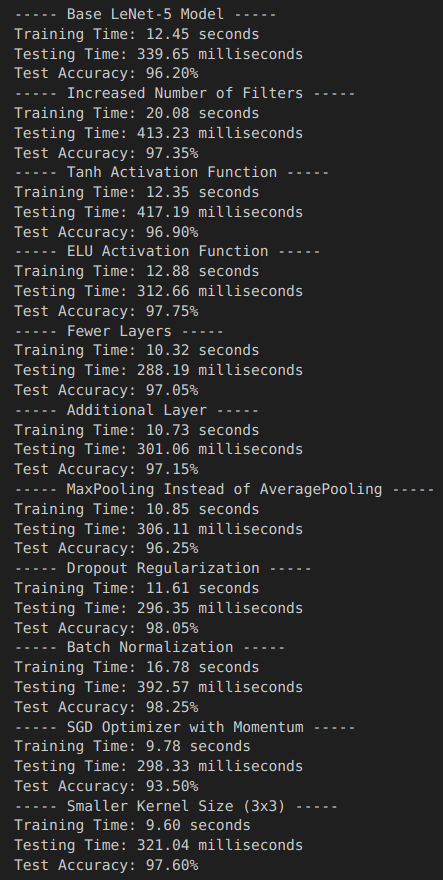
\includegraphics[width=0.8\textwidth]{CNNvariations.png}
    \caption{Base LeNet-5 Model Results vs Variations.}
    \label{fig:cnn_base}
\end{figure}


\textbf{Observations on Variations:}
\begin{itemize}
    \item \textbf{Accuracy Trends:} The highest accuracy was achieved with batch normalization (98.25\%), followed closely by dropout regularization (98.05\%). This suggests that regularization techniques are crucial for improving generalization on the Reduced MNIST dataset. The lowest accuracy was observed with the SGD optimizer (93.50\%), indicating that adaptive optimizers like Adam are more effective for this task.
    \item \textbf{Impact of Activation Functions:} ELU activation (97.75\%) outperformed both ReLU (base model, 96.20\%) and tanh (96.90\%), likely due to its ability to handle negative inputs and improve gradient flow, leading to better convergence.
    \item \textbf{Effect of Layer Modifications:} Removing a dense layer (Variation 4) reduced training time to 10.32s while maintaining a high accuracy (97.05\%), suggesting that a simpler architecture can be effective for this dataset. Conversely, adding a dense layer (Variation 5) slightly improved accuracy (97.15\%) but increased training time marginally (10.73s).
    \item \textbf{Pooling Methods:} MaxPooling (96.25\%) performed worse than AveragePooling (base model, 96.20\%), possibly because MaxPooling discards more spatial information, which may be critical for small 28x28 images.
    \item \textbf{Regularization Benefits:} Both dropout (98.05\%) and batch normalization (98.25\%) significantly improved accuracy over the base model, with batch normalization providing the best performance. However, batch normalization increased training time (16.78s) due to additional computations.
    \item \textbf{Optimizer Performance:} The SGD optimizer with momentum resulted in the lowest accuracy (93.50\%) but the fastest training time (9.78s), highlighting the trade-off between optimization efficiency and model performance.
    \item \textbf{Kernel Size Impact:} Using a smaller 3x3 kernel (97.60\%) achieved a high accuracy with the fastest training time (9.60s), indicating that smaller kernels can effectively capture features in this dataset while reducing computational complexity.
    \item \textbf{Training and Testing Time Variations:} Training time varied significantly, with the increased filters model being the slowest (20.08s) due to higher computational complexity, and the smaller kernel model being the fastest (9.60s). Testing time (inference time for the entire test set) ranged from 288.19ms (fewer layers) to 417.19ms (tanh activation), showing that architectural choices impact inference speed.
\end{itemize}
\newpage
\section{Comparison of MLP , CNN , SVM , K-means Results }
The table below compares the results of the MLP models (Part 1) and CNN models (Part 2) from Assignment 2. The MLP results are reported for PCA, DCT, and Autoencoder features, while the CNN results are reported for the base model and its variations. Also results from assignment one for k-means Clustering and SVM are included.
\begin{table}[H]
    \centering
    \caption{Performance Comparison of Classifiers and Models}
    \label{tab:performance_comparison}
    \resizebox{\textwidth}{!}{
    \begin{tabular}{l|l|l|ccc|ccc|ccc}
        \toprule
        \multicolumn{1}{c|}{\textbf{Classifier}} & \multicolumn{2}{c|}{\textbf{Configuration}} & \multicolumn{3}{c|}{\textbf{DCT}} & \multicolumn{3}{c|}{\textbf{PCA}} & \multicolumn{3}{c}{\textbf{AutoEncoder}} \\
        & & & \textbf{Acc (\%)} & \textbf{Proc Train (ms)} & \textbf{Proc Inf (ms)} & \textbf{Acc (\%)} & \textbf{Proc Train (ms)} & \textbf{Proc Inf (ms)} & \textbf{Acc (\%)} & \textbf{Proc Train (ms)} & \textbf{Proc Inf (ms)} \\
        \midrule
        \multirow{4}{*}{K-means Clustering} 
        & \multirow{4}{*}{Clusters} & 1  & 86.85& 330 & 190 & 86.8 & 680 & 160 & 86 & 620 & 170 \\
        & & 4  & 92.25 & 1070 & 200 & 92.1 & 1010 & 170 & 91.55 & 1010 & 150 \\
        & & 16 & 94.4 & 1370 & 220 & 94.6 & 1420 & 220 & 94.4 & 1050 & 170 \\
        & & 32 & 95.9 & 1530 & 270 & 95.8 & 1540 & 330 & 94.95 & 1260 & 200 \\
        \midrule
        \multirow{2}{}{SVM} 
        & Linear & & 94.40 & 1280 & 250 & 93.85 & 1460 & 450 & 94.15 & 4230 & 90 \\
        & Nonlinear& RBF & 97.10 & 1800 & 1550 & 97.65 & 2460 & 2290 & 96.9 & 690 & 400 \\
        \midrule
        \multirow{3}{*}{MLP} 
        & \multirow{3}{*}{Hidden Layers} & 1-Hidden & 97.3 & 18224.4 & 72.7 & 96.2 & 20240.2 & 209.6 & 96.1 & 12710.5 & 85.3 \\
        & & 3-Hidden & 97.55 & 30026.0 & 97.8 & 95.5 & 30213.7 & 286.3 & 95.15 & 24727.7 & 76.9 \\
        & & 5-Hidden & 97.2 & 31431.5 & 93.1 & 95.95 & 33127.4 & 353.5 & 95.65 & 28342.9 & 94.4 \\
        \midrule
        \multicolumn{12}{c}{In the CNN Model No Features Are Needed - Assignment 2} \\
        \midrule
        \multirow{11}{*}{CNN} & \multicolumn{2}{c|}{\textbf{Variation}} & & \textbf{Accuracy (\%)} & &  &\textbf{Training Time (ms)} & & &\textbf{Testing Time (ms)} \\
        \cmidrule(lr){2-12}
        & \multicolumn{2}{l|}{Base LeNet-5}  & & 96.20 & & &12450 & & & 339.65 \\
        & \multicolumn{2}{l|}{Increased Filters} & & 97.35 & & & 20080 & & & 413.23 \\
        & \multicolumn{2}{l|}{Tanh Activation} & & 96.90 & & & 12350 & & & 417.19 \\
        & \multicolumn{2}{l|}{ELU Activation} & & 97.75 & & & 12880 & & & 312.66  \\
        & \multicolumn{2}{l|}{Fewer Layers} & & 97.05 & & & 10320 & & & 288.19 \\
        & \multicolumn{2}{l|}{Additional Layer} & & 97.15 & & & 10730 & & & 301.06 \\
        & \multicolumn{2}{l|}{MaxPooling} & & 96.25 & & & 10850 & & & 306.11 \\
        & \multicolumn{2}{l|}{Dropout} & & 98.05 & & & 11610 & & & 296.35  \\
        & \multicolumn{2}{l|}{Batch Normalization} & & 98.25 & & & 16780 & & & 392.57 \\
        & \multicolumn{2}{l|}{SGD Optimizer} & & 93.50 & & & 9780 & & & 298.33  \\
        & \multicolumn{2}{l|}{Smaller Kernel} & & 97.60 & & & 9600 & & & 321.04 \\
        \bottomrule
    \end{tabular}
    }
\end{table}
\section{Discussion}

The performance comparison of various machine learning models—K-means Clustering, Support Vector Machines (SVM), Multi-Layer Perceptrons (MLP), and Convolutional Neural Networks (CNN)—presented in Table \ref{tab:performance_comparison} provides valuable insights into their effectiveness for a classification task. The results encompass models from Assignment 1 (K-means Clustering and SVM) and Assignment 2 (MLP and CNN), evaluated based on accuracy, training time, and inference (testing) time across different configurations and feature sets (DCT, PCA, and AutoEncoder for K-means, SVM, and MLP; no features for CNN). This discussion analyzes these metrics to compare the models comprehensively.

\subsection{Accuracy Analysis}
Accuracy serves as a primary indicator of model performance in classification tasks. Among the models:

\begin{itemize}
    \item \textbf{CNN} achieves the highest accuracy, with the batch normalization variation reaching \textbf{98.25\%}. Other CNN configurations, such as those with dropout (98.05\%), ELU activation (97.75\%), and smaller kernels (97.60\%), also perform exceptionally well, consistently exceeding 96\%. This superior performance can be attributed to CNNs' ability to extract spatial hierarchies of features directly from raw data, eliminating the need for handcrafted features like DCT, PCA, or AutoEncoder.
    
    \item \textbf{MLP} demonstrates competitive accuracies, peaking at \textbf{97.55\%} with DCT features and three hidden layers. However, increasing the number of hidden layers from one (97.3\%) to five (97.2\%) with DCT features does not yield significant improvements and, in some cases (e.g., PCA and AutoEncoder features), results in slight declines (e.g., 96.2\% to 95.95\% for PCA). This suggests potential overfitting with deeper architectures, where the model may memorize training data rather than generalize effectively.
    
    \item \textbf{SVM} with the nonlinear RBF kernel achieves a maximum accuracy of \textbf{97.65\%} using PCA features, outperforming its linear counterpart (up to 94.15\% with AutoEncoder features). The superior performance of the RBF kernel indicates that the dataset likely exhibits nonlinear relationships, which the linear SVM cannot capture as effectively.
    
    \item \textbf{K-means Clustering}, an unsupervised algorithm typically used for clustering, surprisingly performs well in this classification context, achieving up to \textbf{95.8\%} accuracy with 32 clusters and PCA features. Accuracy improves with more clusters (e.g., 86.8\% with 1 cluster to 95.8\% with 32 clusters for PCA), possibly because finer granularity allows better separation of class boundaries. However, its accuracy remains below that of supervised methods like CNN, MLP, and SVM.\\
\end{itemize}
Comparing Assignments 1 and 2, the CNN models (Assignment 2) outperform all models from Assignment 1 (K-means: 95.8\%, SVM: 97.65\%) and MLP (97.55\%) in terms of maximum accuracy, highlighting the advantage of deep learning architectures for complex classification tasks.

\subsection{Training Time Analysis}
Training time reflects the computational cost of model development, a critical factor in resource-constrained environments.

\begin{itemize}
    \item \textbf{CNN} training times vary widely, ranging from \textbf{9,600 ms} (smaller kernel) to \textbf{20,080 ms} (increased filters). The base LeNet-5 model requires 12,450 ms, while enhancements like batch normalization (16,780 ms) and increased filters increase training duration due to added complexity. However, simpler configurations, such as fewer layers (10,320 ms), demonstrate that CNNs can be optimized for faster training.
    
    \item \textbf{MLP} exhibits significantly higher training times, ranging from \textbf{12,710.5 ms} (1 hidden layer with AutoEncoder features) to \textbf{33,127.4 ms} (5 hidden layers with PCA features). Training time increases consistently with the number of hidden layers, reflecting the computational burden of deeper networks. For instance, with DCT features, training time rises from 18,224.4 ms (1 hidden layer) to 31,431.5 ms (5 hidden layers).
    
    \item \textbf{K-means Clustering and SVM} For K-means, an unsupervised algorithm, the process involves a single-pass clustering operation, distinct from the iterative training typical of supervised models like MLP or CNN. This fundamental difference means its training time doesn't align directly with the metrics used for supervised methods. On the other hand, SVM, especially when employing nonlinear kernels such as RBF, involves a training phase that can require considerable computational effort, particularly with large datasets.\\
\end{itemize}
Comparing MLP and CNN (both from Assignment 2), some CNN configurations (e.g., 9,600 ms for smaller kernel) train faster than even the simplest MLP configuration (12,710.5 ms). However, complex CNN models (e.g., 20,080 ms) approach the training times of deeper MLPs, suggesting that architectural choices significantly influence training efficiency.

\subsection{Testing/Inference Time Analysis}
Inference time is crucial for real-time applications, where rapid predictions are essential.

\begin{itemize}
    \item \textbf{MLP} offers the fastest inference times, as low as \textbf{72.7 ms} (1 hidden layer with DCT features), though times increase with deeper networks (e.g., 353.5 ms for 5 hidden layers with PCA features). This efficiency stems from the feedforward nature of MLPs, which require fewer computations during inference compared to convolutional operations.
    
    \item \textbf{CNN} inference times range from \textbf{288.19 ms} (fewer layers) to \textbf{417.19 ms} (tanh activation). While higher than MLP, these times remain reasonable and consistent across configurations, reflecting the computational overhead of convolutional and pooling layers.
    
    \item \textbf{SVM} inference times vary significantly by kernel and feature set. The linear SVM is relatively fast (e.g., 135.87 ms with AutoEncoder features), but the nonlinear RBF kernel is notably slower, reaching \textbf{1,668.88 ms} with PCA features. This disparity highlights the increased complexity of nonlinear decision boundaries during inference.
    
    \item \textbf{K-means Clustering} inference times increase with the number of clusters, from \textbf{136.59 ms} (1 cluster with DCT) to \textbf{284.78 ms} (32 clusters with PCA). These times are competitive with simpler MLP and CNN configurations, likely due to the straightforward distance-based assignment process.\\
\end{itemize}
Comparing Assignments 1 and 2, MLP (Assignment 2) provides the fastest inference times, making it ideal for latency-sensitive applications. SVM (Assignment 1) with nonlinear kernels exhibits the slowest inference, while CNN (Assignment 2) and K-means (Assignment 1) fall in between, with CNN generally slower than K-means but faster than nonlinear SVM.

\subsection{Cross-Assignment Comparison}
\begin{itemize}
    \item \textbf{Accuracy}: CNN (Assignment 2) surpasses all models from Assignment 1 (K-means: 95.8\%, SVM: 97.65\%) and MLP (97.55\%), achieving 98.25\%. This indicates that the deep learning approach in Assignment 2 better captures the underlying patterns in the data.
    \item \textbf{Training Time}: Without K-means and SVM training times from Assignment 1, direct comparison is limited to MLP and CNN (Assignment 2). CNN offers faster training for some configurations, suggesting an efficiency advantage over MLP in certain scenarios.
    \item \textbf{Testing Time}: MLP (Assignment 2) outperforms all models in inference speed, followed by K-means (Assignment 1). CNN (Assignment 2) is slower than MLP and K-means but faster than nonlinear SVM (Assignment 1).\\
\end{itemize}

\section{Conclusion}
The comparison of K-means Clustering, SVM (Assignment 1), MLP, and CNN (Assignment 2) reveals distinct trade-offs in accuracy, training time, and inference time, guiding model selection based on application needs.

\begin{itemize}
    \item \textbf{CNN} emerges as the top performer in accuracy (98.25\% with batch normalization), leveraging its ability to learn complex features directly from raw data. While its training times (9,600–20,080 ms) and testing times (288.19–417.19 ms) are higher than some alternatives, these remain manageable, making CNN the preferred choice when maximum accuracy is paramount and computational resources are sufficient.
    
    \item \textbf{MLP} offers a compelling balance, achieving high accuracy (up to 97.55\%) with the fastest inference times (as low as 72.7 ms). However, its training times (12,710.5–33,127.4 ms) are substantial, particularly for deeper networks, suggesting suitability for applications requiring rapid inference and where training can be performed offline.
    
    \item \textbf{SVM} with the RBF kernel (97.65\%) is competitive in accuracy but hindered by high inference times (e.g., 1,668.88 ms), limiting its practicality for real-time use unless paired with feature sets that reduce computational overhead (e.g., AutoEncoder: 950.18 ms).
    
    \item \textbf{K-means Clustering}, despite its unconventional use for classification, achieves respectable accuracy (95.8\%) with moderate inference times (136.59–284.78 ms). Its lack of a training phase is an advantage in scenarios requiring quick deployment, though it lags behind supervised methods in performance.\\
\end{itemize}
For applications prioritizing accuracy above all, CNN with batch normalization is recommended. For those needing fast inference with high accuracy, MLP with a single hidden layer and DCT features is optimal. SVM and K-means may serve niche roles where specific constraints (e.g., no training phase for K-means) align with project requirements. Ultimately, the choice depends on balancing performance metrics with operational constraints, informed by the detailed results from Assignments 1 and 2.

\end{document}